% ============================================================================
%  DRAFT MANUSCRIPT -- prepared for author review, NOT peer reviewed, NOT
%  submitted anywhere. Before submission the authors must:
%    (1) fill in real author names / affiliations / corresponding-author email
%        (placeholders below are marked TODO),
%    (2) verify every bibliography entry against the original source (years,
%        volumes, pages) -- entries below are believed correct but were
%        typeset from memory and are not a substitute for checking,
%    (3) complete the exact citation details marked TODO in the bibliography,
%        and
%    (4) transfer this content into Nature Machine Intelligence's official
%        submission format (they accept a clearly structured Word or PDF
%        document at initial submission). This file uses a plain single-column
%        `article` layout matching their Letters guidelines: unstructured
%        abstract <=150 words, ~3.4k-word main text, 5 display items, Methods
%        after the main text, numbered references, separate Data/Code
%        Availability + Author Contributions + Competing Interests +
%        Acknowledgements sections.
% ============================================================================
\documentclass[11pt]{article}
\usepackage[margin=1in]{geometry}
\usepackage{amsmath,amssymb}
\usepackage{booktabs}
\usepackage{tikz}
\usetikzlibrary{arrows.meta,positioning}
\usepackage[hidelinks]{hyperref}

\newcommand{\zdyn}{\boldsymbol{z}}
\newcommand{\deter}{d}
\newcommand{\stoch}{s}

\begin{document}

\begin{center}
{\LARGE\bfseries Stable and verifiable latent dynamics for world models}\\[0.6em]
{\large [TODO: Author Name(s)]}\\[0.2em]
{\normalsize [TODO: Affiliation, Department, Institution, City, Country]}\\[0.2em]
{\small [TODO: corresponding author email]}
\end{center}

\begin{abstract}
\noindent
World models of the Dreamer family optimize policies over latent trajectories
imagined by a recurrent state-space model, yet nothing in their training
constrains those latent dynamics to be stable, and the categorical latent
output blocks direct formal certification. We report two measured obstacles
and an evaluation standard for the resulting problem. First, a
sampling-to-proof gap audit of the one-step latent map under a frozen actor:
a Lyapunov decrease condition, a large random-sampling baseline, and
branch-and-bound verification with a reachability gate. Second, a measured
verifier wall: interval bound propagation asserts on the categorical output
at any useful width, so every branch-and-bound box is recorded as
\emph{unknown} with its reason, never as a violation. Third, a five-mode
failure atlas from a controlled latent-space study shows why naive stability
constraints fail, from which we derive design rules and an
aliveness-gated evaluation standard. All claims name the object, region, and
condition that produced them.
\end{abstract}

% =====================================================================
\section{Introduction}

Model-based reinforcement learning via world models has become a general
approach to control. DreamerV3~\cite{hafner2025nature,hafner2023arxiv}
masters over 150 tasks from a single configuration, and its policy is
optimized over trajectories \emph{imagined in latent space} by a Recurrent
State-Space Model (RSSM)~\cite{hafner2019icml} -- never in the environment.
This is precisely why the stability of the latent dynamics matters: if the
imagined trajectory drifts off-distribution, diverges, or collapses to a
spurious fixed point, the policy is optimized against a model of a world
that does not exist. DreamerV3 is trained with no constraint that the latent
transition map be contractive, energy-bounded, or otherwise stable, and its
categorical latent output complicates any formal argument about the imagined
dynamics.

Two lines of work have begun to address this. The first constrains the
\emph{learned} dynamics so imagination stays well behaved; the most recent
example is Koopman Dreamer~\cite{koopman2026}, which replaces the
deterministic latent core with spectrally constrained rotation--scaling
blocks of bounded radius and derives a multi-step rollout-error bound. The
second verifies a \emph{frozen} model after the fact with neural Lyapunov
methods~\cite{chang2019,dawson2023} and sound bound
propagation~\cite{zhang2018crown,xu2020autolirpa}. Both lines face a common,
largely unexamined question: how large is the gap between what random
sampling finds and what a verifier can prove, and can scalar or spectral
constraints actually shape the stability of a learned latent map?

This Letter reports three measured results on that question. (i) A
sampling-to-proof gap audit for the one-step latent map of a DreamerV3-size
model under a frozen actor. (ii) A structural verifier wall: interval bound
propagation cannot bind the categorical latent output at any useful width.
(iii) A five-mode failure atlas, from a controlled latent-space study, of
how the optimizer routes around scalar stability constraints -- including
the decoupling of spectrum-sum constraints from the leading Lyapunov
exponent and the decoupling of finite-time spectral proxies from the
asymptotic exponent. From the atlas we derive design rules for stabilization
attempts and an evaluation standard that gates attractor-overlap metrics on
rollout aliveness.

\emph{Honest framing.} This is a methods and measurement Letter. The verifier
wall and the failure atlas are measured; the direct application to a
\emph{trained} DreamerV3 on a control task is [TODO: pending GPU audit], and
no quantitative claim about DreamerV3 itself is made until that audit lands.
The latent-space study uses Lorenz-63, which is not a natural GENERIC
system; its learned energy and dissipation are proxies. We claim
on-attractor stability and invariant recovery, not recovery of true
thermodynamics.

% =====================================================================
\section{The one-step latent map and the sampling-to-proof gap audit}

DreamerV3's world model factorizes the transition into a deterministic
recurrent core and a stochastic posterior over discrete
classes: $\deter_t = f_\theta(\deter_{t-1}, \stoch_{t-1}, a_{t-1})$ and
$\stoch_t \sim q_\phi(\stoch_t \mid \deter_t, o_t)$, with a prior
$p_\phi(\stoch_t \mid \deter_t)$ used at imagination time. The object we
audit is the one-step latent map under a frozen deterministic actor
$\pi$,
\begin{equation}
  \label{eq:onestep}
  \zdyn = (\deter, \stoch) \;\mapsto\;
  \zdyn' = \big(\deter',\; \mathrm{softmax}(\mathrm{logits}')\big),
  \qquad \deter' = \mathrm{core}\big(\deter, \pi(\zdyn)\big),
\end{equation}
where the stochastic output is replaced by the \emph{mean} of the prior
categorical, and $\pi(\zdyn) = \tanh(\mathrm{mean}(\mathrm{actor}))$. The
model is audited as trained; only the Lyapunov candidate $V$ moves. Nothing
about the imagined multi-step rollout is certified, and nothing larger than
the size-1M configuration (deter 512, hidden 64, stoch $32\times4$) is
considered.

The audit (Fig.~\ref{fig:pipeline}) verifies the Lyapunov decrease condition
\begin{equation}
  \label{eq:cond}
  \mathrm{cond}(\zdyn) = V(\zdyn) - V(\zdyn') > 0
\end{equation}
over a box region built \emph{from} the model's own latent states: a frozen
checkpoint is rolled out on-policy, the posterior latents are recorded, and
the certified region is the coordinate box around them. The region is
therefore on-distribution by construction; the certified map is the
prior-mean surrogate, and the distinction is recorded in the artifact, never
conflated.

Sampling draws $\zdyn$ uniformly from the box and evaluates
Eq.~\eqref{eq:cond} exactly. Branch-and-bound uses CROWN-style
relaxations~\cite{zhang2018crown} as implemented in
auto\_LiRPA~\cite{xu2020autolirpa}, with the verifier source pinned by the
SHA-256 of the driver. A verdict is one of three: \emph{violation} (a
counterexample the model demonstrably reaches), \emph{certified} (the bound
proves the condition on the whole box), or \emph{unknown} (bounds stayed
loose, no counterexample found). \emph{Unknown} is verifier incompleteness:
it is never evidence of safety, and it is never a gap and never a partial
finding. The branch-and-bound region is an annulus around the latent fixed
point $\zdyn^*$, holed along the $k$ coordinate dimensions with the largest
halfwidths so the number of boxes scales with $k$, not with the latent
dimension; the fixed point itself, where $\mathrm{cond}(\zdyn^*) = 0$ by
construction, is excluded.

\begin{figure}[t]
\centering
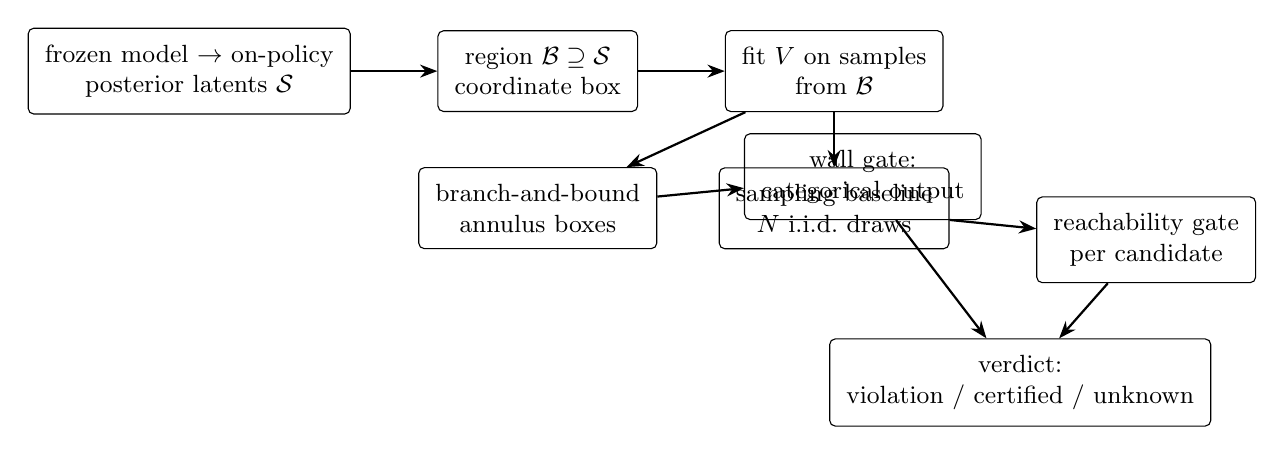
\begin{tikzpicture}[
  node distance=1.1cm,
  box/.style={draw, rounded corners=2pt, align=center, inner sep=6pt,
              font=\small, minimum height=1.4em},
  arr/.style={-{Stealth[length=2.2mm]}, thick},
]
\node[box] (sup) {frozen model $\to$ on-policy\\posterior latents $\mathcal{S}$};
\node[box, right=of sup] (reg) {region $\mathcal{B}\supseteq\mathcal{S}$\\coordinate box};
\node[box, right=of reg] (V) {fit $V$ on samples\\from $\mathcal{B}$};
\node[box, below=0.7cm of V] (sam) {sampling baseline\\$N$ i.i.d.\ draws};
\node[box, below=0.7cm of reg] (bab) {branch-and-bound\\annulus boxes};
\node[box, right=of sam, yshift=-0.4cm] (gate) {reachability gate\\per candidate};
\node[box, right=of bab, yshift=0.4cm] (wall) {wall gate:\\categorical output};
\node[box, below=0.7cm of gate, xshift=-1.6cm] (verdict)
      {verdict:\\ violation / certified / unknown};
\draw[arr] (sup) -- (reg);
\draw[arr] (reg) -- (V);
\draw[arr] (V) -- (sam);
\draw[arr] (V) -- (bab);
\draw[arr] (bab) -- (wall);
\draw[arr] (wall) -- (verdict);
\draw[arr] (sam) -- (gate);
\draw[arr] (gate) -- (verdict);
\end{tikzpicture}
\caption{The sampling-to-proof gap audit. The region is built from the
model's own on-policy latents; sampling and branch-and-bound compete on the
same decrease condition; candidates pass a reachability gate; a structural
wall probe records boxes that the verifier cannot bind.}
\label{fig:pipeline}
\end{figure}

% =====================================================================
\section{The verifier wall on categorical latents}

The certified graph contains the categorical output
$\stoch' = \mathrm{softmax}(\mathrm{logits}')$, i.e.\ an
$\exp/\sum\exp$ with a division by the relaxed sum. Interval bound
propagation asserts on this node whenever the relaxed logits interval spans a
region where the softmax denominator can be non-positive in the bound
computation; at the measured vacuity of the intermediate bounds this happens
on the first box (``AssertionError in BoundReciprocal''), and the same
structural failure repeats identically on every box. Because the bound-graph
build dominates the per-box cost (measured: $\sim$4 minutes for the graph
trace on a size-1M graph on CPU), running branch-and-bound without the wall
gate wastes hours to rediscover the same assertion.

The audit therefore probes the wall once, then records every box as
\emph{unknown} with the reason ``categorical output not interval-bindable at
this width''. This is the toolchain boundary, now \emph{measured} rather
than assumed. The sampling baseline is the empirical result, and a sampling
violation is the only thing that can become a finding; it must survive the
reachability gate first.

On the smoke configuration -- a weight-initialized surrogate, \emph{not} a
trained model -- the full pipeline runs end to end on CPU
(Table~\ref{tab:smoke}). \emph{None of these numbers describe a trained
model}; they establish that the pipeline is sound and reproducible, which is
their only claim. The trained-model audit on dm\_control cartpole\_balance
is [TODO: pending GPU]; on the categorical wall its expected verdict is
\emph{unknown}, which is verifier incompleteness and not a finding.

\begin{table}[t]
\centering
\caption{Measured audit record on the smoke configuration
(weight-initialized surrogate; CPU; not a trained model).}
\label{tab:smoke}
\small
\begin{tabular}{@{}ll@{}}
\toprule
Quantity & Measured \\
\midrule
Latent fixed point residual & $2.98\times10^{-8}$ (converged) \\
Region coverage of steady-state latents & 83.8\% \\
Sampling baseline & 0 / 12\,866 violations \\
Worst sampling condition & $+2.2\times10^{-3}$ \\
Branch-and-bound boxes & 4 (k-dim hole) \\
Wall record & every box \emph{unknown}: categorical output \\
Verdict & $\texttt{gap\_demonstrated} = \mathtt{false}$ \\
\bottomrule
\end{tabular}
\end{table}

% =====================================================================
\section{The failure atlas of latent-space stabilization}

The wall says the frozen model cannot be certified directly. The remaining
question is whether it can be \emph{stabilized} -- and here we report the
atlas from a controlled study: a Hamiltonian-JEPA predictor trained end to
end on chaotic Lorenz-63 under a nonlinear coordinate warp, in five ablation
arms with matched data and steps (unconstrained MLP; rigid Hamiltonian;
naive metriplectic; fixed divergence-free-$J$ metriplectic with invariant
dissipation gate; and the fixed arm plus a differentiable QR spectral
alignment). The study is reproducible on CPU with fixed seeds. The atlas is
the \emph{negative result}: imposing physical or thermodynamic constraints
inside a self-supervised latent space does not, by itself, yield physical
dynamics, because the optimizer routes around each scalar constraint through
a geometric exploit (Table~\ref{tab:atlas}).

\begin{table}[t]
\centering
\caption{Documented failure modes of latent-space stabilization
(Lorenz-63, nonlinear warp; signatures as documented, CPU reproduction in
progress at draft time).}
\label{tab:atlas}
\small
\begin{tabular}{@{}lll@{}}
\toprule
\# & Mode & Measured signature \\
\midrule
1 & Representation freeze &
  motion $\sim10^{-3}$ vs target $\sim0.4$; penalty $\sim0$ \\
2 & Scale-conditioning paradox &
  proxy spread $\sim0.036$ vs $\|\partial H/\partial p\| \sim 3.2$ \\
3 & Skew loophole + dead R saddle &
  $\mathrm{tr}(R)/n = 0.00000$ in every naive run \\
4 & Sum-vs-$\lambda_1$ decoupling &
  contraction $-12.8$, $\lambda_1$ blows up to $+3.5$ (true $\sim0.88$) \\
5 & Finite-time spectral trap &
  short-horizon $\hat\lambda_1 \to -0.17$, true 200-step $+1.44$ \\
\bottomrule
\end{tabular}
\end{table}

\textbf{(1) Freeze.} Multi-step alignment is minimized by a predictor that
does not move: compounding $K$-step error makes motion locally costlier than
none, and the field gradients collapse. A horizon curriculum and a detached
motion-magnitude penalty are partial mitigations.

\textbf{(2) Scale-conditioning paradox.} Matching the raw magnitude of a
kinetic-energy proxy clamps the dynamics: the proxy's spread is
$\sim30\times$ below what the integrator needs, so magnitude matching
freezes the model. Comparing \emph{z-scores} of both sides -- keeping only
the shape/correlation constraint -- restores an $O(1)$ loss and frees the
scale.

\textbf{(3) Skew loophole and dead R saddle.} A state-dependent skew
$\mathbf{J}(\zdyn)$ is not divergence-free, so it can supply demanded volume
contraction with no dissipation at all, leaving $\mathbf{R}$ off; and
$\mathbf{R} = \mathbf{L}\mathbf{L}^\top$ with $\mathbf{L}$ zero-initialized
has $\partial\mathbf{R}/\partial\mathbf{L} = 0$ at $\mathbf{L}=0$, a dead
saddle no gradient can lift. Both must be closed -- fixed constant canonical
skew, small nonzero $\mathbf{L}$ init -- before dissipation engages
($\mathrm{tr}(R)/n \sim 5.6$; contraction $-13.667$).

\textbf{(4) Sum-vs-$\lambda_1$ decoupling.} Pinning the divergence pins the
\emph{sum} of the Lyapunov spectrum, but the sum does not pin any individual
exponent. The fixed arm reaches strong contraction while $\lambda_1$ blows
up to $+3.5$ (true $\sim0.88$): the negative exponents compensate. Confirmed
four times ($\lambda_1 \in \{-0.42, +1.44, +3.5, +4.29\}$, all with the
``correct'' sum). A scalar volume constraint is structurally incapable of
shaping the leading exponent -- the direct caution for spectral designs that
constrain aggregate spectrum information, such as bounded-radius
backbones~\cite{koopman2026}.

\textbf{(5) Finite-time spectral trap.} At short horizons the finite-time QR
exponent decouples from the asymptotic $\lambda_1$: training drives
$\hat\lambda_1$ to $-0.17$ while the true 200-step exponent is $+1.44$
(opposite sign). At long horizons the proxy is trainable but nothing
constrains global boundedness: the evaluation rollout diverges to
$+\infty$. The trap moves from ``wrong proxy'' to ``right proxy, unbounded
global trajectory''.

\textbf{The overlap trap (evaluation standard).} Chamfer/Hausdorff distance
to the encoded attractor \emph{rewards} a frozen predictor: a stationary
point inside the attractor cloud scores near-perfect while being dynamically
dead. Geometric overlap must be gated on the rollout being alive and chaotic
($\lambda_1 > 0$ and a sane motion ratio), or replaced by a
motion-invariant statistic.

\emph{Transfer caveat.} The atlas is measured on Lorenz-63 latent dynamics,
not on DreamerV3's RSSM latents. Its role here is to make the failure modes
concrete and checkable; the audit of Section~2 is the tool that tests
whether the same exploits appear in a trained world model's latent space.
That test is the primary open item.

% =====================================================================
\section{Design rules and the evaluation standard}

From the wall and the atlas we derive the following rules; each is stated
with the failure mode it is designed to avoid (Table~\ref{tab:rules}).

\begin{enumerate}
\item \textbf{Certify a verifiable surrogate, not the categorical output.}
The categorical output is not interval-bindable at useful width. Certification
must target the deterministic component of the latent map, or a structurally
verifiable surrogate, with the stochastic output treated as the documented
boundary of the toolchain.
\item \textbf{Constrain modes, not sums.} A scalar volume/spectrum-sum
constraint cannot shape the leading Lyapunov exponent. Spectral designs
should constrain per-mode radii and verify the \emph{leading} exponent
directly, not the aggregate.
\item \textbf{Break dead saddles with principled initialization.} Factorized
dissipation or learned structure that starts at zero and is penalized toward
engagement needs a nonzero initialization and a gradient-path check.
\item \textbf{Use shape constraints, not raw magnitudes.} Scale-free
(z-score/correlation) anchors decouple magnitude from shape and prevent
scale-starvation.
\item \textbf{Curriculize the horizon and gate evaluation on aliveness.}
Short-horizon objectives freeze the predictor, and finite-time proxies
decouple from asymptotic exponents; evaluation must include a long-horizon
rollout, an aliveness gate, and a leading-exponent check, and must never
report attractor overlap without it.
\item \textbf{Report the gap honestly.} \emph{Unknown} verdicts, loose
bounds, and walls are verifier incompleteness: never evidence of safety,
never a gap. Only a reachable violation counts, and it must survive a
reachability gate.
\end{enumerate}

\begin{table}[t]
\centering
\caption{Design rules for stabilizing latent dynamics, indexed by the
failure mode each avoids.}
\label{tab:rules}
\small
\begin{tabular}{@{}ll@{}}
\toprule
Rule & Avoids \\
\midrule
Certify a verifiable surrogate & categorical wall (Section 3) \\
Constrain modes, not sums & failure 4 (sum-vs-$\lambda_1$) \\
Break dead saddles with init & failure 3 (dead R saddle) \\
Shape constraints, not magnitudes & failure 2 (scale paradox) \\
Curriculize horizon; gate on aliveness & failures 1 and 5; overlap trap \\
Report unknown honestly & overstatement \\
\bottomrule
\end{tabular}
\end{table}

\begin{figure}[t]
\centering
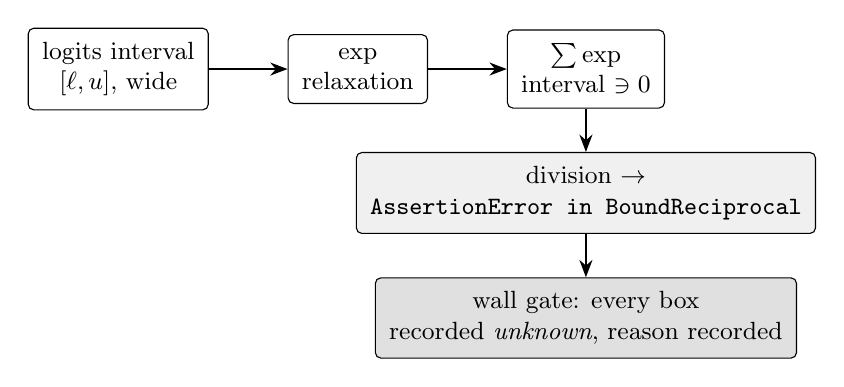
\begin{tikzpicture}[
  node distance=1.0cm,
  box/.style={draw, rounded corners=2pt, align=center, inner sep=5pt,
              font=\small},
  arr/.style={-{Stealth[length=2.2mm]}, thick},
]
\node[box] (l) {logits interval\\$[\ell, u]$, wide};
\node[box, right=of l] (e) {$\exp$\\relaxation};
\node[box, right=of e] (s) {$\sum\exp$\\interval $\ni 0$};
\node[box, below=0.55cm of s, fill=black!6] (r) {division $\to$\\
  \texttt{AssertionError in BoundReciprocal}};
\node[box, below=0.55cm of r, fill=black!12] (w) {wall gate: every box\\
  recorded \emph{unknown}, reason recorded};
\draw[arr] (l) -- (e);
\draw[arr] (e) -- (s);
\draw[arr] (s) -- (r);
\draw[arr] (r) -- (w);
\end{tikzpicture}
\caption{The measured categorical wall. The softmax / sum-division node
asserts in the interval pass at any useful width, so the audit probes once
and records every box as \emph{unknown} with its reason.}
\label{fig:wall}
\end{figure}

% =====================================================================
\section{Discussion}

\emph{What is measured.} The verifier wall is a measured property of
auto\_LiRPA~0.7.2 on the categorical output, reproducible on CPU in minutes.
The failure atlas is a measured, reproducible negative result on a
controlled latent-space benchmark. The audit pipeline is measured end to end
on a surrogate.

\emph{What is not yet measured.} A trained DreamerV3 model's latent dynamics
have not yet been audited; that audit requires a GPU training run and is the
primary open item. The transfer of the failure modes from Lorenz latents to
RSSM latents is a hypothesis the audit is designed to test, not a claim.
\emph{Unknown} verdicts on the categorical wall are expected and are not
findings.

\emph{Scope.} The certified object is the one-step prior-mean map under a
frozen policy; nothing about imagined multi-step rollouts or the stochastic
posterior is certified. The region is built from on-policy posterior
latents; the certified map is the prior-mean surrogate.

\emph{Implications for the field.} World-model-based control deployed on
physical systems needs latent trajectories that stay bounded and
on-distribution over planning horizons, and a way to argue about that
formally. This Letter contributes the measurement machinery (the gap audit),
the obstacle (the categorical wall), and the cautionary evidence (the
failure atlas) that any stabilization design must confront. We do not claim
to know any team's internal priorities; we claim only that these are the
questions any stability argument for a Dreamer-style latent space must
answer.

% =====================================================================
\section{Methods}

\textbf{Audit procedure.} The pipeline (Fig.~\ref{fig:pipeline}) is: fit the
Lyapunov candidate $V$ by gradient descent on samples from the region
(penalizing violations of Eq.~\eqref{eq:cond}); run the sampling baseline
($N$ i.i.d.\ draws, worst condition and count recorded); run
branch-and-bound over the annulus boxes with a per-box budget; apply the
reachability gate to any candidate violation by simulating the model's
closed-loop dynamics toward it; probe the categorical wall once and record
unbindable boxes as \emph{unknown} with the reason. The verdict is
$\texttt{gap\_demonstrated}$ only when sampling found nothing and
branch-and-bound found a reachable violation.

\textbf{Region construction.} A frozen checkpoint is rolled out on-policy;
posterior latents are recorded; the region is the coordinate box around
them. The annulus excludes the latent fixed point and is holed along the $k$
coordinate dimensions with the largest halfwidths.

\textbf{Verifier pinning.} The verifier is auto\_LiRPA~0.7.2 at GitHub commit
5a098e8f (the release the project was validated against; PyPI releases carry
incompatible legacy torch constraints). The driver that produced a result is
pinned by the SHA-256 of its source. The categorical wall is probed by a
single structural test of the interval pass on the softmax/sum-division node.

\textbf{Latent-space benchmark.} Lorenz-63 ($\sigma=10$, $\rho=28$,
$\beta=8/3$) is sampled at $\mathrm{d}t=0.01$, lifted by a fixed nonlinear
diffeomorphism into a 64-D latent space, and predicted by five JEPA
predictor arms (unconstrained MLP; rigid Hamiltonian; naive metriplectic;
fixed-$J$ metriplectic with invariant dissipation gate; fixed arm plus
differentiable QR spectral alignment), each trained with matched data,
steps, and seeds. Evaluation is a 200-step rollout judged by boundedness,
leading Lyapunov exponent (Benettin), phase-space contraction rate,
attractor overlap (Hausdorff/Chamfer), and dissipation engagement
$\mathrm{tr}(R)/n$. The empirical true exponent at $\mathrm{d}t=0.01$ is
$+0.884$ (textbook $0.9056$); the true divergence is $-13.6667$. All
reported numbers come from fixed-seed runs; per-seed spread is reported
where available.

\textbf{Code and data availability.} The audit pipeline, the port of the
DreamerV3 size-1M networks, the notebook builder, and this manuscript are in
the public repository github.com/sehajr-singhs/rl-wm-audit. The failure
atlas benchmark, results, and figures are in
github.com/sehajr-singhs/spectral-topological-decoupling. All code runs on
CPU.

% =====================================================================
\section*{Data and Code Availability}
See Methods.

\section*{Author Contributions}
[TODO]

\section*{Competing Interests}
The authors declare no competing interests.

\section*{Acknowledgements}
[TODO]

\begin{thebibliography}{99}

\bibitem{hafner2025nature}
D.~Hafner, J.~Pasukonis, J.~Ba, and T.~Lillicrap,
``Mastering diverse control tasks through world models,''
\emph{Nature}, vol.~[TODO], 2025. [TODO: verify volume/pages/DOI.]

\bibitem{hafner2023arxiv}
D.~Hafner, J.~Pasukonis, J.~Ba, and T.~Lillicrap,
``Mastering diverse domains through world models,''
arXiv preprint arXiv:2301.04104, 2023.

\bibitem{hafner2019icml}
D.~Hafner, T.~Lillicrap, I.~Fischer, R.~Villegas, D.~Ha, and H.~Lee,
``Learning latent dynamics for planning from pixels,''
in \emph{Proc. ICML}, 2019.

\bibitem{koopman2026}
J.~Li, X.~Zhang, H.~Xie, Y.~Lan, W.~Pan, and X.~Xu,
``Koopman Dreamer: Spectrally constrained latent dynamics for stable
world-model imagination,''
arXiv preprint arXiv:2607.19719, 2026.

\bibitem{zhang2018crown}
H.~Zhang, T.-W.~Weng, P.-Y.~Chen, C.-J.~Hsieh, and L.~Daniel,
``Efficient neural network robustness certification with general activation
functions,''
in \emph{Proc. NeurIPS}, 2018.

\bibitem{xu2020autolirpa}
K.~Xu, \emph{et al.},
``auto\_LiRPA: Automatic linear relaxation based perturbation analysis for
neural networks,''
arXiv preprint arXiv:2002.12920, 2020.

\bibitem{chang2019}
Y.-C.~Chang, N.~Roohi, and S.~Gao,
``Neural Lyapunov control,''
in \emph{Proc. NeurIPS}, 2019.

\bibitem{dawson2023}
C.~Dawson, S.~Gao, and C.~Fan,
``Safe control with learned certificates: A survey of neural Lyapunov,
barrier, and contraction methods,''
arXiv preprint arXiv:2202.11762, 2023.

\bibitem{lecun2022pathway}
Y.~LeCun,
``A path towards autonomous machine intelligence,''
Open Review preprint, 2022.

\bibitem{assran2023self}
M.~Assran, \emph{et al.},
``Self-supervised learning from images with a joint-embedding predictive
architecture,''
in \emph{Proc. CVPR}, 2023.

\bibitem{maes2026}
L.~Maes, Q.~Le~Lidec, D.~Scieur, Y.~LeCun, and R.~Balestriero,
``LeWorldModel: Stable end-to-end joint-embedding predictive architecture
from pixels,''
arXiv preprint arXiv:2603.19312, 2026.

\bibitem{miller2019}
J.~Miller and M.~Hardt,
``Stable recurrent models,''
in \emph{Proc. ICLR}, 2019.

\end{thebibliography}

\vspace{1em}
\noindent\textbf{Draft status.} Authors TODO; references to verify; the
trained-model audit [TODO: GPU run]; the CPU reproduction of the atlas table
in progress at draft time. Nothing in this draft has been submitted or peer
reviewed.

\end{document}
